\begin{outline-text-1}
\begin{xlarge}
\begin{center}
今日の話: いろいろ
\end{center}
\end{xlarge}

\begin{center}
東京大学 総合文化研究科 D2 浅井 政太郎
\end{center}

\begin{note}
\begin{alignright}
Made by guicho2.71828 (Masataro Asai)
\end{alignright}
\end{note}
\end{outline-text-1}

\section{近況報告 ICAPS 2016 @ London (Intl. Conf. Automated Planning \& Scheduling)}
\label{sec-1}

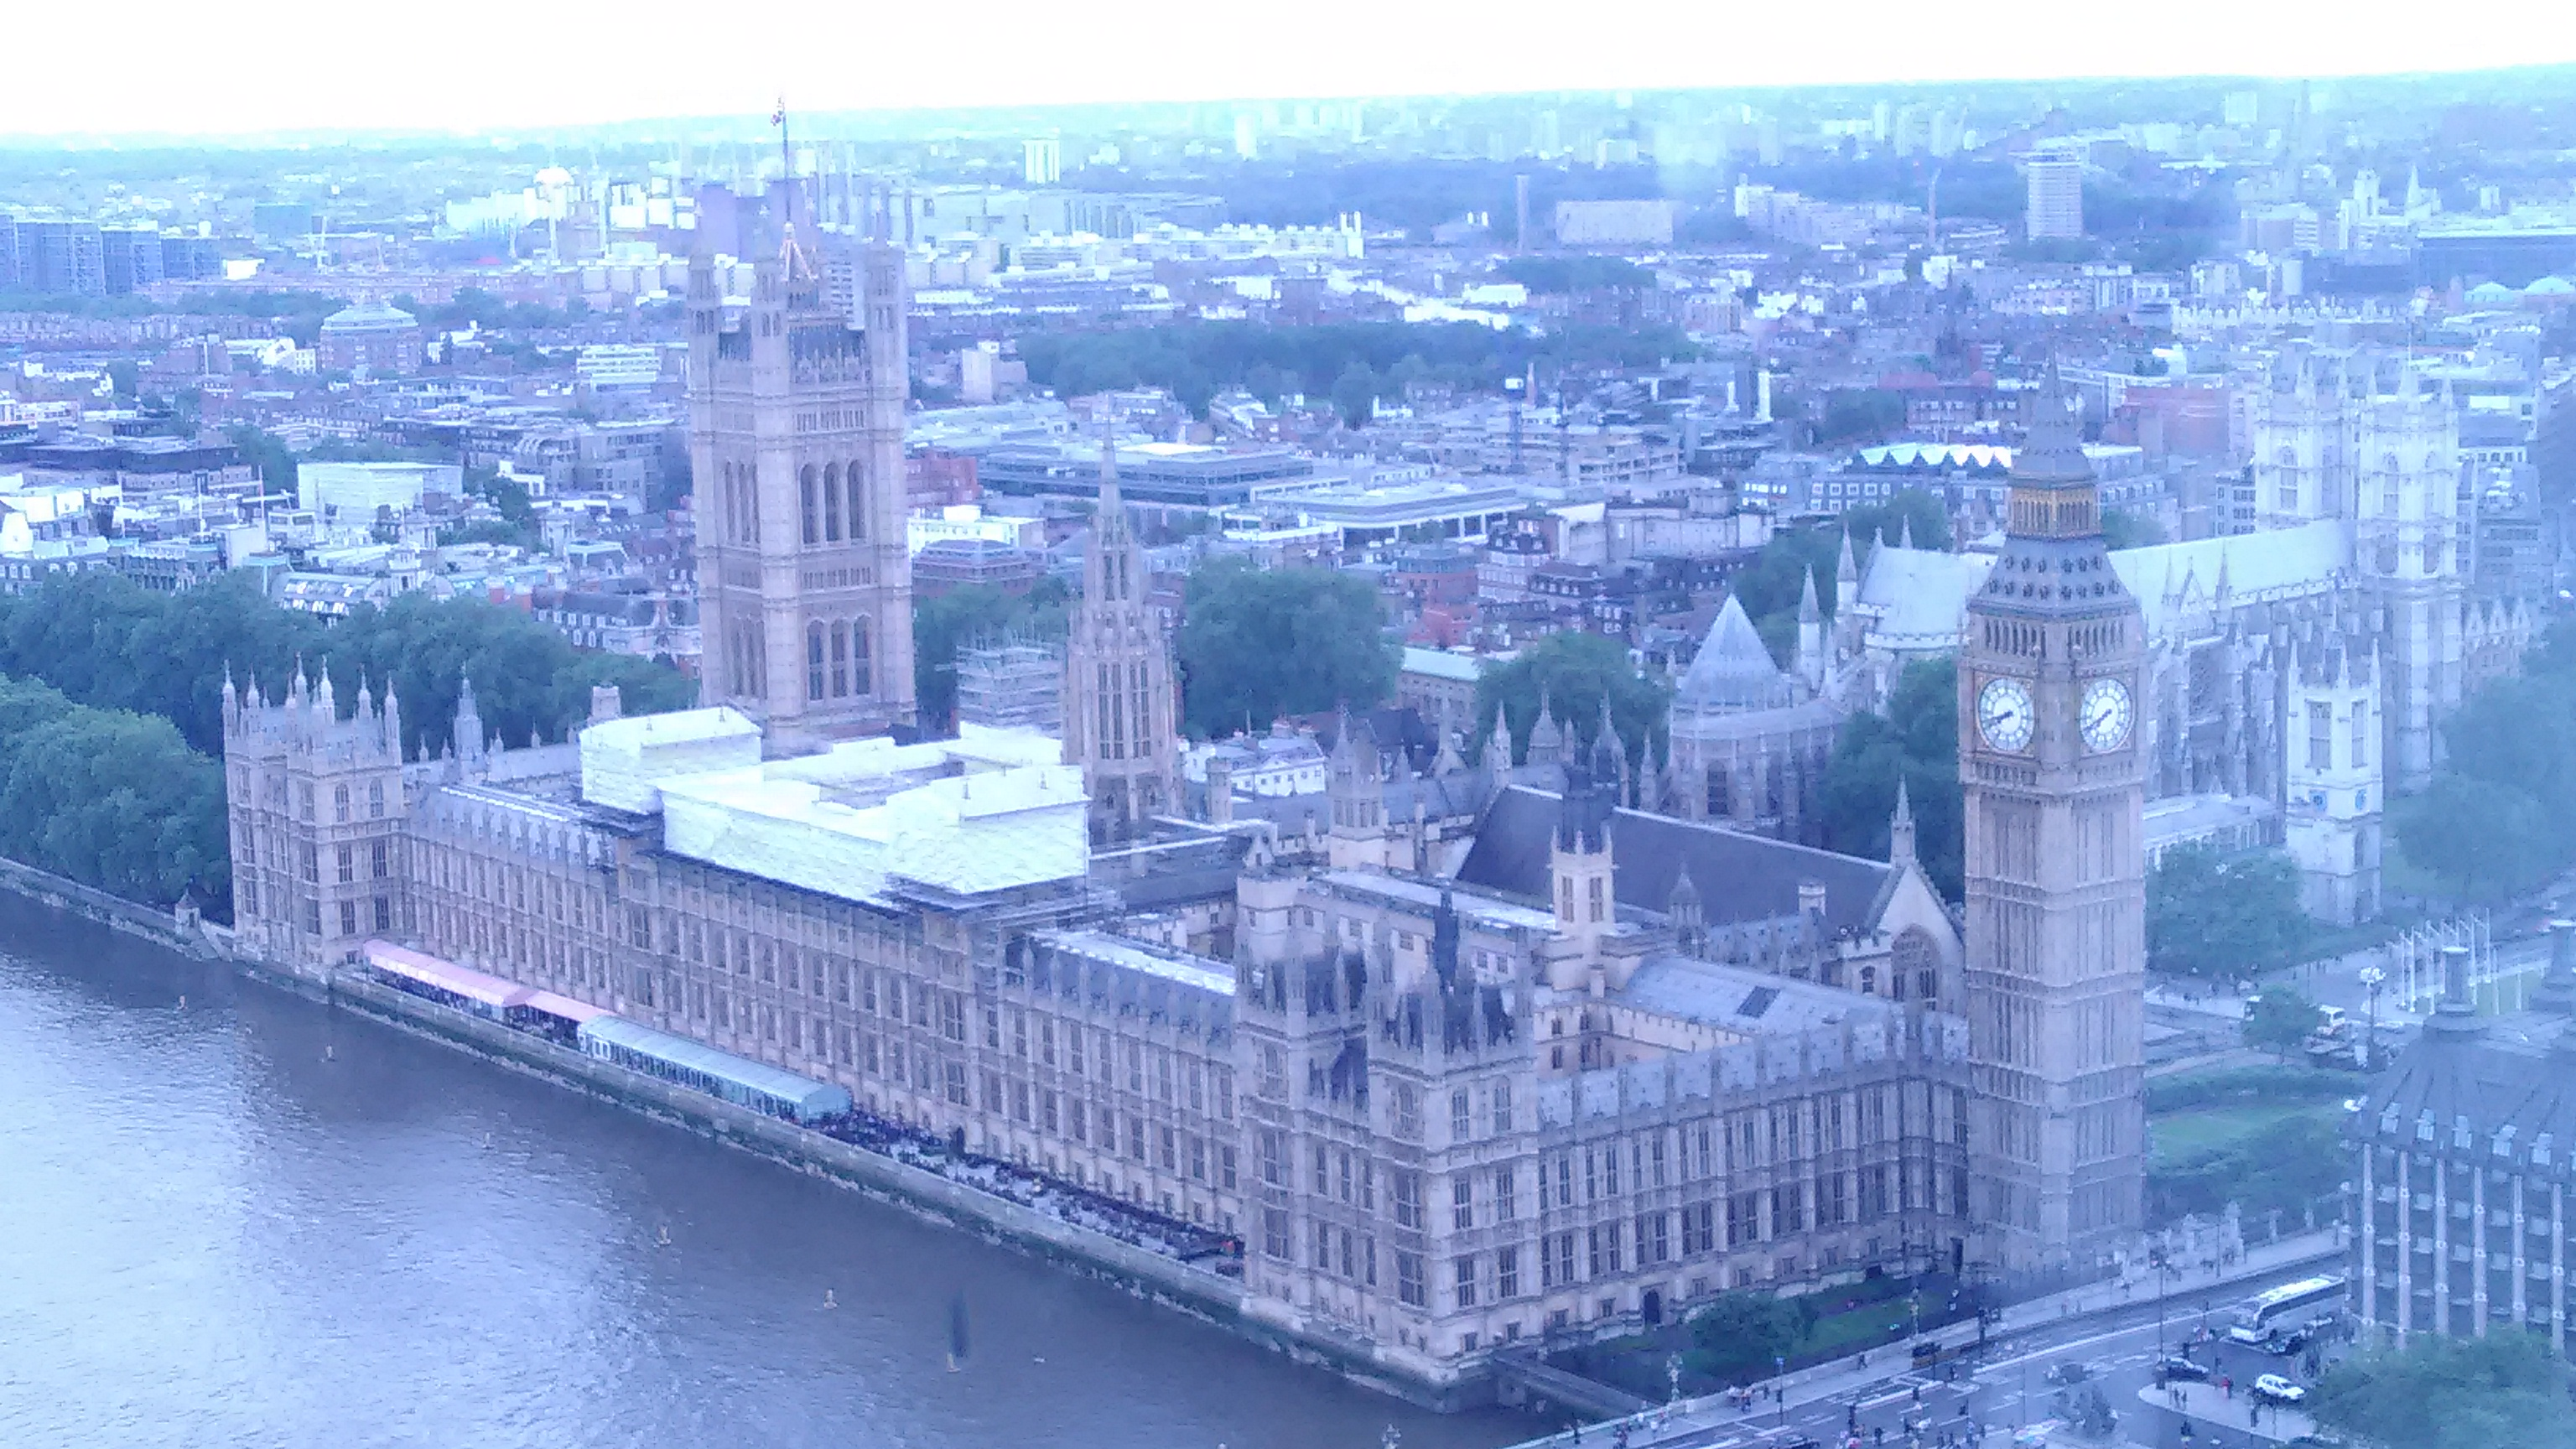
\includegraphics{img/static/bigben.jpg}

\section{MIT Lispers}
\label{sec-2}



\section{フライトが長い}
\label{sec-3}

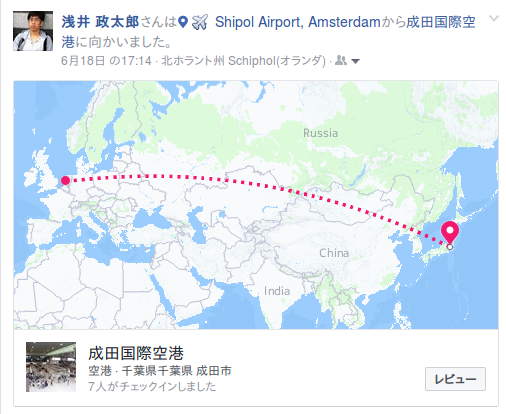
\includegraphics{img/static/flight.png}

\begin{xlarge}
\begin{alignright}
\begin{itemize}
\item なにかつくろう!
\end{itemize}
\end{alignright}
\end{xlarge}

\section{}
\label{sec-4}

\begin{xlarge}
\begin{center}
成果
\end{center}
\end{xlarge}

\section{Hypercast -- なんでも変換機}
\label{sec-5}

\begin{larger}
\begin{verbatim}
(cast 5 'bit-vector)
; -> #*1010000000000000000000000000000000000000000000000000000000000000
\end{verbatim}
\end{larger}

\begin{enumerate}
\item \texttt{cl:coerce} 互換
\item Inlined CLOS で生成 → 定数引数であればコンパイル時にディスパッチ
\item 自動型変換 → 型変換の経路を自動探索
\end{enumerate}

\section{cl:coerce}
\label{sec-6}
